\documentclass[11pt]{article}

\usepackage[utf8]{inputenc}
\usepackage[T1]{fontenc}
\usepackage[margin=1in]{geometry}
\usepackage{amsmath}
\usepackage{amssymb}
\usepackage{graphicx}
\graphicspath{{../}}
\usepackage{hyperref}
\usepackage{xcolor}
\usepackage{enumitem}

\hypersetup{
  colorlinks=true,
  linkcolor=blue!50!black,
  citecolor=blue!50!black,
  urlcolor=blue!50!black,
  pdftitle={Some Mathematics behind elbow-helper},
  pdfauthor={Warith Harchaoui}
}

\usepackage[round]{natbib}
\bibliographystyle{plainnat}

\newcommand{\code}[1]{\texttt{#1}}

\title{Some Mathematics behind \code{elbow-helper}}
\author{Warith Harchaoui}
\date{Summer 2026}

\begin{document}
\maketitle

\begin{abstract}
This note explains, from first principles, every piece of mathematics
\code{elbow-helper} runs: the shipped single-knee pipeline
(\code{robust\_knee}, \code{robust\_elbow}) and the multi-knee research
behind \code{robust\_knees}. Citations live in \code{references.bib}; each
claim states whether it is a verified citation, a citation reported through
a secondary source, or this project's own construction, following the
evidence-marking convention used throughout this project.

\textbf{How to read this note.} Every concept gets the same treatment: first
a plain-language explanation with a concrete example, assuming nothing
beyond high-school algebra; then the precise formula, for a reader who wants
to check every step, including a reader with a Ph.D.\ in applied mathematics
who wants to verify the derivation rather than trust the prose. Skip the
formula blocks on a first pass if the intuition already answers your
question. Come back to them when it doesn't.

The note is organized around a single question, asked three times with
increasing realism: what does \emph{one} knee mean geometrically
(Part~\ref{part:one}), what does \emph{several} knees mean geometrically
(Part~\ref{part:several}), and how do you trust either answer once the data
is noisy (Part~\ref{part:noise})?
\end{abstract}

\clearpage

\tableofcontents

\clearpage

\part{Introduction}
\label{sec:intro}

A knee or an elbow, on a curve of diminishing returns, marks the point
past which more input stops buying much more output. Existing detectors
are good at proposing where that point sits; what they lack is a notion
of confidence, so a single point estimate on a noisy curve is easy to
over-trust in practice. \code{elbow-helper} wraps a from-scratch locator
in a conservative decision procedure and refuses to answer outright when
the evidence is weak.

This note derives, from first principles, every piece of mathematics the
package runs. Several of its model-selection criteria, scores that reward
a good fit while penalizing extra complexity, trace back to the same
Gaussian log-likelihood: single-knee $\mathrm{BIC}$, the Bayesian
Information Criterion (Section~\ref{sec:bic-cv}); the several-knee
$\mathrm{BIC}(k)$ of Section~\ref{sec:several-bic}; its stricter cousin
the modified Bayesian Information Criterion, $\mathrm{mBIC}$
(Section~\ref{sec:mbic}); and a version that also charges for ambiguous
segment boundaries, the Integrated Completed Likelihood, $\mathrm{ICL}$
(Section~\ref{sec:icl}). This Introduction derives that shared foundation
once, in natural log throughout, before any of those sections adds its
own penalty term on top.

\section{From raw likelihood to a bounded score}
\label{sec:likelihood-intro}

Start from the raw likelihood, before taking any logarithm at all, and
take it \emph{per observation} from the outset: the geometric mean of the
$n$ individual Gaussian densities, rather than their raw product. Under a
generative model $y_i = f(x_i;\theta) + \varepsilon_i$ with $\varepsilon_i$
i.i.d.\ $\mathcal N(0,\sigma^2)$ ($f$ any of the curve models this note
fits, a single line, a broken line, or a $k$-segment piecewise line;
$\theta$ its shape parameters):

\begin{equation}
L(\theta,\sigma^2) := \left(\prod_{i=1}^n (2\pi\sigma^2)^{-1/2}
\exp\!\left(-\frac{(y_i - f(x_i;\theta))^2}{2\sigma^2}\right)\right)^{1/n}
\end{equation}

The product of $n$ identical prefactors and the product of exponentials
both collapse cleanly under the $1/n$ root: a product of exponentials is
an exponential of a sum, and that sum divided by $n$ is a mean.

\begin{equation}
L(\theta,\sigma^2) = (2\pi\sigma^2)^{-1/2}
\exp\!\left(-\frac{1}{2\sigma^2}\cdot\frac{1}{n}\sum_{i=1}^n (y_i - f(x_i;\theta))^2\right)
= (2\pi\sigma^2)^{-1/2}\exp\!\left(-\frac{\mathrm{MSE}(\theta)}{2\sigma^2}\right)
\end{equation}

the average per-point squared error, the mean squared error
$\mathrm{MSE}(\theta) := \frac{1}{n}\sum_i (y_i - f(x_i;\theta))^2$.
$L$ is already an $\exp$ expression, base $e$, straight from the Gaussian
density's own definition, before any analyst chooses to take a logarithm
for convenience. Taking $\ln$ of $L$ therefore does not introduce a base;
it undoes the one already there:

\begin{equation}
\ell(\theta,\sigma^2) := \ln L(\theta,\sigma^2)
= -\frac{1}{2}\ln(2\pi\sigma^2) - \frac{\mathrm{MSE}(\theta)}{2\sigma^2}
\end{equation}

Minimizing $\mathrm{MSE}$ over $\theta$ at fixed $\sigma^2$ is maximizing
$\ell$ over $\theta$, the reason ordinary least squares and Gaussian
maximum likelihood are one procedure, not two. Profiling out $\sigma^2$ at
its best-supported value, the maximum likelihood estimate (MLE)
$\hat\sigma^2 = \mathrm{MSE}$, and exponentiating $-2\ell$, the
conventional scaling for an information criterion, undoes the $\ln$ and
lands on a single clean per-observation quantity, the measure information
theory calls perplexity:

\begin{equation}
\mathrm{PPL}(\theta) := \exp\!\big(-2\,\ell(\theta,\hat\sigma^2)\big) = 2\pi e \cdot \mathrm{MSE}(\theta)
\end{equation}

Scaling this per-observation perplexity back up to the full $n$-point
sample recovers the negative log-likelihood, $\mathrm{NLL}$, every
$\mathrm{BIC}$-family formula in this note is built from, written here
through the residual sum of squares, $RSS(\theta) := \sum_i (y_i -
f(x_i;\theta))^2$, the un-averaged numerator $\mathrm{MSE}$ divides by
$n$:

\begin{equation}
\mathrm{NLL} := n \ln \mathrm{PPL}(\theta) = n \ln\!\left(\frac{RSS}{n}\right) + n(1 + \ln 2\pi)
\end{equation}

the same $n\ln(RSS/n)$ term every $\mathrm{BIC}$-family formula in this
note opens with.

\textbf{Extreme cases, without a sigmoid.} $\mathrm{PPL}$ is a genuine
improvement over the raw $\mathrm{NLL}$ it is built from at exactly one
end: $\mathrm{NLL}$ runs over $(-\infty, +\infty)$, but exponentiating
automatically fixes the lower tail, $\mathrm{PPL} = 2\pi e \cdot
\mathrm{MSE}(\theta) \ge 0$ always, with $\mathrm{PPL} = 0$ at a perfect
fit ($\mathrm{MSE} \to 0$): the Gaussian degeneracy behind BIC's whole
reason to exist, a model with as many parameters as points drives
$\mathrm{MSE}$ to zero and its raw likelihood to infinity. The upper end
is still unresolved: $\mathrm{MSE} \to \infty$ is not a meaningful worst
case; it is merely unbounded, not a real reference point any fit would
sit near. The sample
mean $\bar y$ is not a good worst-case reference either: it is the
\emph{unique} constant that \emph{minimizes} $\mathrm{MSE}$ among all
constants, the best trivial predictor there is, not a bad one. That is
exactly why normalizing against it (the textbook $R^2$) can still go
negative: a real fit is easy to make worse than the one constant nothing
else can beat. A genuinely pessimistic, finite worst case instead picks
the single \emph{observed} point that is hardest to predict everything
else from:

\begin{equation}
y_{\text{bad}} := \operatorname*{arg\,max}_{y_j \in \{y_1,\dots,y_n\}}
\frac{1}{n}\sum_i (y_i - y_j)^2, \qquad
\mathrm{MSE}_{\text{worst}} := \frac{1}{n}\sum_i (y_i - y_{\text{bad}})^2
\end{equation}

Since $\bar y$ uniquely minimizes $\mathrm{MSE}$ among constants, any other
constant, an actual observed value most of all, scores strictly worse:
$\mathrm{MSE}_{\text{worst}} > \mathrm{Var}(y)$ always. Normalizing against
this harder-to-beat ceiling instead,

\begin{equation}
1 - \frac{\mathrm{MSE}(\theta)}{\mathrm{MSE}_{\text{worst}}} = 1 - \frac{\mathrm{PPL}(\theta)}{\mathrm{PPL}_{\text{worst}}}
\end{equation}

gives a score anchored at $1$ for a perfect fit and at $0$ for a fit
exactly as bad as $y_{\text{bad}}$ itself, with a far higher bar to cross
into negative territory than the mean-based $R^2$ ever offers, since
$\mathrm{MSE}_{\text{worst}} > \mathrm{Var}(y)$ by construction, built
entirely from $\mathrm{MSE}$ against a real, deliberately pessimistic
reference point, with no Bayes factor or posterior probability anywhere
in the derivation. This is a stricter cousin of $R^2$, not $R^2$ itself,
$R^2$ keeps $\bar y$ as its baseline and accepts the occasional negative
score in exchange. \code{elbow\_helper.plotting}'s diagnostic legend takes
a different route again, converting $\Delta\mathrm{BIC}$ directly into a
posterior probability via a Bayes factor \citep{kassraftery1995}, a valid
alternative normalization built on the same $\mathrm{NLL}$ but not the one
derived here.

Every $\mathrm{BIC}$-family quantity in this note inherits this same
natural-log base by construction: each is $\mathrm{NLL}$ plus a complexity
penalty, never a likelihood rederived from scratch. Changing the log base
anywhere downstream would mean rederiving the Gaussian density itself in
that base, not rescaling a finished number.

\section{Related Work}
\label{sec:related-work}

\textbf{Knee and elbow heuristics.} Satopaa, Albrecht, Irwin and
Raghavan's Kneedle \citep{satopaa2011} locates a knee via the same
difference-from-chord geometry Section~\ref{sec:diff-curve} builds on, as
a single point estimate with no confidence machinery.
\code{elbow-helper}'s locator borrows that geometric intuition and wraps
it in the decision procedure this note derives.

\textbf{Changepoint detection and segmentation.} Killick, Fearnhead and
Eckley's pruned dynamic-programming algorithm, Pruned Exact Linear Time
(PELT) \citep{killick2012}, achieves exact, optimal segmentation at linear
cost, the same optimal-substructure principle Section~\ref{sec:dp} is
built on too, restricted here to a small $k_{\max}$ rather than PELT's
penalty-driven unbounded $k$. Fryzlewicz's
Wild Binary Segmentation \citep{fryzlewicz2014} is the greedy alternative
to exact dynamic programming behind Section~\ref{sec:greedy}'s comparison.
Yao \citep{yao1988} first analyzed estimating the number of changepoints
via Schwarz's criterion, the direct ancestor of the several-knee
$\mathrm{BIC}(k)$ criterion in Section~\ref{sec:several-bic}.

\textbf{Model selection criteria.} Schwarz \citep{schwarz1978} is
$\mathrm{BIC}$'s origin. Zhang and Siegmund \citep{zhangsiegmund2007}
correct $\mathrm{BIC}$'s undercharging for breakpoint-location freedom,
the $\mathrm{mBIC}$ of Section~\ref{sec:mbic}. Biernacki, Celeux and
Govaert \citep{biernacki2000} introduce the Integrated Completed
Likelihood for mixture models, adapted to changepoints in
Section~\ref{sec:icl} via Rigaill, Lebarbier and Robin's exact
forward-backward posterior over segmentations \citep{rigaill2012},
further accelerated by Cleynen, Luong, Rigaill and Nuel
\citep{cleynen2013}. Kass and Raftery \citep{kassraftery1995} supply the
Bayes-factor route from a raw likelihood difference to a posterior
probability, the alternative normalization noted above.

\textbf{Sequential and multiscale testing.} Davies \citep{davies1977}
addresses hypothesis testing when a nuisance parameter, here the
breakpoint location, exists only under the alternative, a problem
Section~\ref{sec:fwer}'s sequential test runs into directly. Frick, Munk
and Sieling's Simultaneous MUlti-scale Change-point Estimator (SMUCE)
\citep{frick2014} gives the same kind of guarantee across every scale at
once, cited alongside it.

\textbf{Robust and classical statistics.} Spearman's rank correlation
\citep{spearman1904} screens for a monotonic trend before any knee search
runs. Theil \citep{theil1950} and Sen \citep{sen1968} give the
outlier-robust slope estimator behind the Theil-Sen contrast check.
Efron's bootstrap \citep{efron1979} is the resampling method behind the
stability check.

\textbf{Methodology.} L\'opez de Prado \citep{lopezdeprado2018financial}
argues at length for contiguous, not shuffled, cross-validation on
ordered sequential data, the reasoning behind this project's blocked
cross-validation.

\textbf{Further reading.} Hastie, Tibshirani and Friedman
\citep{hastie2009esl}, Bishop \citep{bishop2006prml}, Bouveyron, Celeux,
Murphy and Raftery \citep{bouveyron2021mbc}, Cormen, Leiserson, Rivest and
Stein \citep{cormen2022algorithms}, and Dasgupta, Papadimitriou and
Vazirani \citep{dasgupta2006algorithms} are cited throughout as accessible
textbook treatments, not as the origin of any specific claim above; a few,
drawn from the author's own curated
\href{https://deraison.ai/ai-books}{book list}, are pointed to only where
directly relevant.

\clearpage

\part{One knee, the geometry of a bend}
\label{part:one}

\section{Putting the data on common ground: normalization}

\textbf{Intuition.} A curve of website visits over months and a curve of
stock prices over years look nothing alike numerically: one might range over
thousands, the other over single digits, yet both could share the same
\emph{shape}. Before comparing shapes, both axes get rescaled into the same
box, the unit square $[0,1] \times [0,1]$, so every threshold used later in
the pipeline --- how sharp a bend counts, how much noise is too much ---
means the same thing regardless of the data's original units.

\textbf{Formula.} $x$ is scaled linearly:

\begin{equation}
x_{\text{norm}} = \frac{x - x_{\min}}{x_{\max} - x_{\min}}
\end{equation}

$y$ is scaled the same way, but using the 5th and 95th percentiles instead
of the raw minimum and maximum, then clipped to $[0,1]$:

\begin{equation}
y_{\text{scaled}} = \operatorname{clip}\!\left(\frac{y - y_{p5}}{y_{p95} - y_{p5}},\ 0,\ 1\right)
\end{equation}

The percentile choice is not cosmetic: a single wild outlier, a data-entry
error, a one-off spike, would otherwise stretch the whole $y$ axis to
accommodate it, crushing the real signal into a sliver near zero.
Percentiles absorb a handful of extreme points without distorting the shape
that matters (\code{src/elbow\_helper/preprocessing.py}).

\section{The difference-curve bump: what ``knee'' means, exactly}
\label{sec:diff-curve}

\textbf{Intuition.} A textbook knee, shaped like $\sqrt{x}$, rises fast then
levels off. Subtracting the straight diagonal line joining the curve's two
endpoints from the curve itself produces a bump: it starts at zero, peaks
somewhere in the middle, and returns to zero. The peak of that bump sits
exactly where the curve bends hardest away from a straight line, which is
the intuitive definition of a ``knee''. This picture turns into an algorithm
\citep{satopaa2011}: subtract the diagonal, find the bump's peak, call it the
knee. \code{elbow-helper}'s \code{locator.py} is a from-scratch NumPy port;
see the project's \code{README.md} Acknowledgements section for the
implementation's origin.

Four shapes exist in principle --- concave-increasing, concave-decreasing,
convex-increasing, convex-decreasing --- but only one of them,
concave-increasing, is the ``obvious'' bump-above-the-diagonal case.
\code{elbow-helper} reorients the other three into that one case first
(flip, mirror, or both, depending on \code{curve}/\code{direction}), runs
the same bump-peak logic, then un-transforms the answer. This is why
\code{curve} and \code{direction} matter: they tell the algorithm which of
the four mirror images it is looking at.

\textbf{Formula.} After orienting to the concave-increasing frame, the
difference curve is

\begin{equation}
d(x_i) = y_{\text{norm}}(x_i) - x_{\text{norm}, i}
\end{equation}

Its local maxima are candidate knees. At each local maximum $j$, a
sensitivity threshold controls how far the curve must dip below the peak
before that peak is trusted as a real knee rather than a wiggle:

\begin{equation}
T_j = d_{\max, j} - S \cdot \overline{|\Delta x_{\text{norm}}|}
\end{equation}

where $S$ is the sensitivity parameter: a larger $S$ is more conservative,
demanding a bigger dip. The bar denotes the mean spacing between consecutive
$x$ values. Traversing the difference curve left to right, a knee is
declared at the last index before $d(x)$ drops below the currently active
threshold $T_j$; in ``online'' mode the traversal keeps re-arming at every
later, higher peak, so only the last, most persistent bump wins
(\code{src/elbow\_helper/locator.py}, \code{find\_knee}).

\section{The broken-line model: a knee as a change of slope}

\textbf{Intuition.} A real knee should let a two-piece line --- straight,
then a different straight slope after the knee --- fit the data noticeably
better than a single straight line can. \code{elbow-helper} builds that
two-piece model as one continuous curve using a hinge function, $\max(0, x -
k)$, which is exactly zero before the knee $k$ and grows linearly after it,
so adding it to a plain line produces a single formula for a line that
bends at $k$ without jumping:

\begin{equation}
y = a + b\,x + c \cdot \max(0,\ x - k)
\end{equation}

This is the algebraic object every confirmation check in
Part~\ref{part:noise} is ultimately built around: fitting it by ordinary
least squares and comparing its residual error against a plain line's
answers the question ``does a bend here actually help''.

\section{A worked example: the k-means inertia elbow}

\code{robust\_elbow}'s own docstring names this the flagship
convex-decreasing case, and it is worth seeing end to end: run k-means for
$k = 1, 2, \dots$, plot the inertia (within-cluster sum of squared
distances) against $k$, and look for the point past which adding another
cluster stops paying for itself.

\code{tests/test\_real\_world\_examples.py::\allowbreak kmeans\_inertia\_curve} builds
eight well-separated 2D blobs, each its own mildly elongated ellipse rather
than a plain isotropic Gaussian, and runs Lloyd's algorithm (fifteen random
restarts per $k$, to avoid a bad local optimum blurring the curve) for $k =
1, \dots, 24$. Inertia falls by two orders of magnitude at $k = 8$, the true
cluster count. What happens after $k = 8$ is the point worth looking at
closely: inertia keeps decaying, gently and a little unevenly, rather than
snapping flat. That leftover slope is real, not noise in the plotting
sense: each blob's own elongation gives a $k$ past 8 a little genuine
sub-structure to exploit, exactly as a real dataset's clusters are never
perfect circles either. The figure below plots inertia on a logarithmic
axis for this reason: the drop at $k=8$ is so much larger than the tail's
own gentle decay that a linear axis would flatten the tail to the eye even
though the underlying numbers keep falling.

\textbf{Reading the evidence legend, ahead of its own derivation.} The
figure below is this note's first with the full diagnostic legend
\code{elbow\_helper.plotting} draws next to every confirmed knee, five
numbers Parts~\ref{part:several}--\ref{part:noise} derive properly later;
in plain language ahead of that: \emph{detection probability}
(Section~\ref{sec:bootstrap}) is how often the identical knee reappears
under a residual bootstrap redo: close to $100\%$ means the knee is not
an artefact of this one particular noise draw. \emph{null p} (null
$p$-value, Section~\ref{sec:null-test}) is how surprising the observed
knee would be if the true curve were a straight line: small means a
straight-line explanation is implausible. \emph{slope contrast}
(Section~\ref{sec:theilsen}) is a $[0,1]$ score for how sharply the slope
actually changes at the knee: near $100\%$ means the two sides point in
essentially opposite or wildly different directions. \emph{posterior
probability} (Section~\ref{sec:bic-cv}) is the BIC-derived odds, under a
Bayes-factor approximation, that a broken line genuinely fits better than
a single straight one rather than by chance. \emph{fit quality}
(Section~\ref{sec:likelihood-intro}, already derived) is how close the
confirmed broken-line fit sits to the data relative to a deliberately
pessimistic worst case: $100\%$ at a perfect fit. Every one of the five
is a bounded, justified $[0,1]$ score, not a raw, scale-dependent
statistic a reader has to calibrate by eye; four read strong evidence as
a number near $100\%$, only null $p$ runs the other way, small rather
than large, exactly a $p$-value's usual convention.

\begin{figure}[h]
\centering
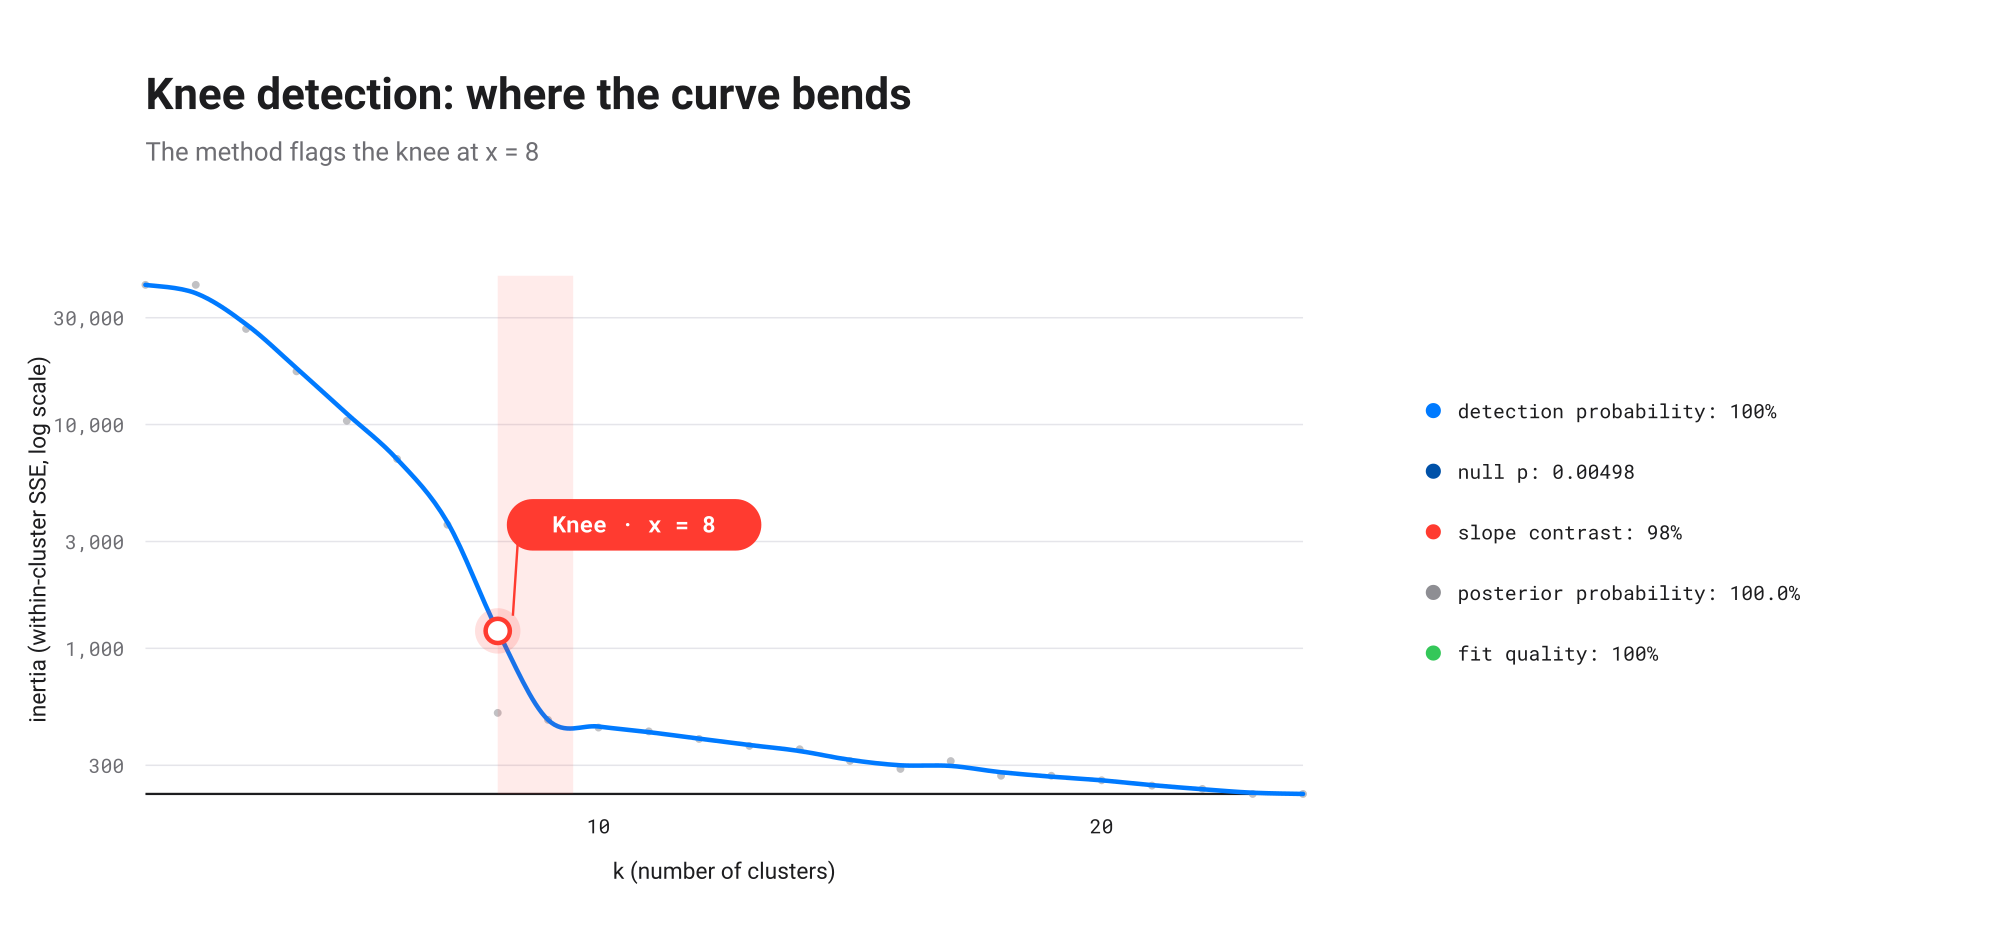
\includegraphics[width=0.8\textwidth]{figures/kmeans_en.png}
\caption{The k-means inertia curve on a log-scale y-axis, with
\code{elbow\_helper.robust\_elbow}'s detected elbow (dashed red line) at
k=8, the true number of clusters, and a gently decaying tail past it.}
\end{figure}

\textbf{Two practical traps this example surfaced, worth stating plainly.}
First: a k-means inertia curve has one point per candidate $k$, rarely more
than a couple of dozen, and its genuine elbow usually sits close to the
\emph{left} edge, at a small $k$, not in the middle. \code{elbow-helper}'s
defaults (Sections~\ref{sec:multiscale}--\ref{sec:null-test}) are calibrated
for longer, noisier, elbow-anywhere measurement curves:
\code{min\_samples=20} and \code{min\_side\_points=5} reject a short,
left-heavy curve like this one outright.
\code{tests/test\_real\_world\_examples.py} ships a \code{RobustKneeConfig}
profile with both of those relaxed, plus several of the persistence and
bootstrap thresholds loosened to match, and states in a comment exactly why:
short, clean applied curves are a genuinely different regime from the long,
noisy time-series-like curves the defaults target, not a bug in either.
Second: blocked cross-validation (Section~\ref{sec:bic-cv}) splits a curve
this short, about 25 points, into \code{cv\_folds} contiguous pieces, and
the default of 5 folds leaves so few points per fold that a fold boundary
landing near the elbow can flip the sign of the held-out improvement on an
unlucky seed. Three wider folds instead of five fixes it, a direct,
checkable illustration of Section~\ref{sec:bic-cv}'s own point that
cross-validation needs enough data per fold to say anything stable.

\part{Several knees, the geometry of many bends}
\label{part:several}

\section{The model: independent linear segments}

\textbf{Intuition.} Cut the curve into pieces at $k$ breakpoints and fit
each piece its own straight line, independently, allowing a visible jump at
each cut rather than forcing the pieces to meet exactly. This is a
deliberate departure from Part~\ref{part:one}'s continuous hinge model: once
more than one breakpoint is free to move, a \emph{continuous}
piecewise-linear fit no longer decomposes into a sum of independent
per-piece costs --- moving one breakpoint changes the boundary condition
every neighbouring piece must satisfy. That dependency breaks the efficient
search algorithms below. The changepoint literature this section draws on
and tests --- Yao, Zhang and Siegmund, PELT, binary segmentation --- is
stated for independent segments, so matching that model is what makes the
comparison a fair test of \emph{their} claims, not a test of a different
model wearing their name.

\section{Segment cost, in closed form}

\textbf{Intuition.} Fitting a straight line through a handful of points and
measuring how well it fits, the residual sum of squares (RSS), sounds like
it should be done point by point, but a shortcut exists: once five running
totals are known --- a sum of $x$'s, of $y$'s, of $x^2$'s, of $xy$'s, of
$y^2$'s --- the best-fit line's RSS for \emph{any} stretch of points can be
computed in one step, without touching the individual points again.
Precomputing those totals once, then reading off any segment's cost
instantly, is what makes searching over thousands of ways to cut the curve
computationally realistic.

\textbf{Formula.} For a segment covering $m$ points with values $x_1,
\dots, x_m$ and $y_1, \dots, y_m$, let

\begin{equation}
S_1 = m,\quad S_x = \sum_i x_i,\quad S_y = \sum_i y_i,\quad S_{xx} = \sum_i x_i^2,\quad S_{xy} = \sum_i x_i y_i,\quad S_{yy} = \sum_i y_i^2
\end{equation}

The least-squares slope and intercept of $y = a + bx$ are

\begin{equation}
b = \frac{m\,S_{xy} - S_x S_y}{m\,S_{xx} - S_x^2}, \qquad a = \frac{S_y - b\,S_x}{m}
\end{equation}

and, substituting into $RSS = \sum_i (y_i - a - b x_i)^2$ and simplifying
with the normal equations,

\begin{equation}
RSS = S_{yy} - a\,S_y - b\,S_{xy}
\end{equation}

Precomputing the six running sums once costs $O(n)$; every later
segment-cost lookup then costs $O(1)$. This is standard practice in
changepoint software, a direct algebraic consequence of the least-squares
normal equations, not a result that needs its own citation.

\section{Optimal partitioning: the dynamic program}
\label{sec:dp}

\textbf{Intuition.} Choosing the single best way to place $k$ breakpoints
among $n$ points by trying every combination would be astronomically slow.
Dynamic programming avoids this by building the answer from smaller
sub-answers: the cheapest way to explain the first $t$ points with $k$
segments is, for every possible location of the last cut $s$, the cheapest
way to explain the first $s$ points with $k-1$ segments, plus the cost of
one final segment from $s$ to $t$, minimized over all valid $s$. Because the
best $k$-segment answer depends only on the best $(k-1)$-segment answers,
each already computed once, no combination is ever recomputed. This is
Bellman's principle of optimality.

\textbf{Formula.} With $C[k][t]$ the minimal total RSS of the first $t$
points cut into $k+1$ segments:

\begin{equation}
C[0][t] = \operatorname{cost}(0, t)
\end{equation}
\begin{equation}
C[k][t] = \min_{s} \Big( C[k-1][s] + \operatorname{cost}(s, t) \Big)
\end{equation}

where $s$ ranges over cut points that leave every segment at least
\code{min\_seg} points long. Solving this for every $k$ up to $k_{\max}$ and
every $t$ up to $n$ costs $O(k_{\max} \cdot n^2)$, each cell an $O(n)$
minimization over $O(1)$ segment costs from the previous section.
Backpointers recover the actual cut positions.
\code{research/multiknee/tests/test\_segmentation.py::\allowbreak test\_dp\_matches\_brute\_force\_small\_n}
checks this against literal enumeration of every valid partition on small
inputs, so its correctness is verified empirically, not just asserted from
the textbook recursion \citep{cormen2022algorithms,dasgupta2006algorithms}.

This is the same recursion underlying Yao \citeyearpar{yao1988}, Zhang and
Siegmund \citeyearpar{zhangsiegmund2007}, and PELT, ``Pruned Exact Linear
Time'', due to Killick, Fearnhead and Eckley \citeyearpar{killick2012}. PELT
is this recursion with a pruning step added that provably never removes the
optimum for an additive penalty, so it returns identical answers, only
faster. No separate PELT implementation was built for that reason: it would
reproduce these numbers exactly.

\section{Greedy binary segmentation: the faster, worse alternative}
\label{sec:greedy}

\textbf{Intuition.} Instead of solving the whole problem exactly,
repeatedly make the single best choice available right now: find the one
split that most reduces the \emph{global} error, commit to it, then repeat
on the two resulting pieces. This is much faster than the dynamic program,
but it can only ever produce worse or equal outcomes, never better, because
it locks in early decisions before later evidence exists to correct them.

\textbf{A concrete failure, not a hypothetical one.}
\code{research/multiknee/tests/test\_segmentation.py::\allowbreak test\_greedy\_can\_strictly[...]noiseless}
exhibits a noiseless curve with two sharp, real breakpoints where greedy's
\emph{first} split lands on neither of them; by the time greedy adds a
second split, it still has strictly higher error than the dynamic program's
exact, zero-error optimum. \code{research/multiknee/RESULTS.md} measures
the downstream consequence directly: every DP-based method beats its greedy
counterpart. Greedy's early-commitment errors specifically cause it to
\emph{overselect} the number of breakpoints at low noise, since fixing
greedy's own placement mistake later looks, to a model-selection criterion,
like genuine extra structure worth an extra breakpoint. This is the
textbook motivation for Wild Binary Segmentation \citep{fryzlewicz2014}.

\section{A worked example: a mountain of alternating slopes}

Part~\ref{part:one}'s \code{robust\_knee} needs \code{curve}/\code{direction}
to know which of the four mirror images it is looking at, or must infer it
from the whole curve's global shape. A curve that goes up, flattens, comes
back down, and flattens again, a mountain, has no single global shape at
all: Section~4's fixed-sign geometry cannot describe it, no matter how
\code{curve}/\code{direction} are set.

\code{robust\_knees} sidesteps the question entirely, because this part's
independent-segment model never assumes a shared sign for the slopes in the
first place: each segment gets its own free slope, so a sign change from
one segment to the next is not a special case, just what the data happens
to show.

\code{tests/test\_multiknee.py::\allowbreak alternating\_slope\_curve} builds exactly
this: steep up, flat, steep down, flat, four segments and three
breakpoints, each a genuine sign or magnitude change. \code{robust\_knees}
recovers all three, in the right order, with the right signs, on every seed
tested.

\begin{figure}[h]
\centering
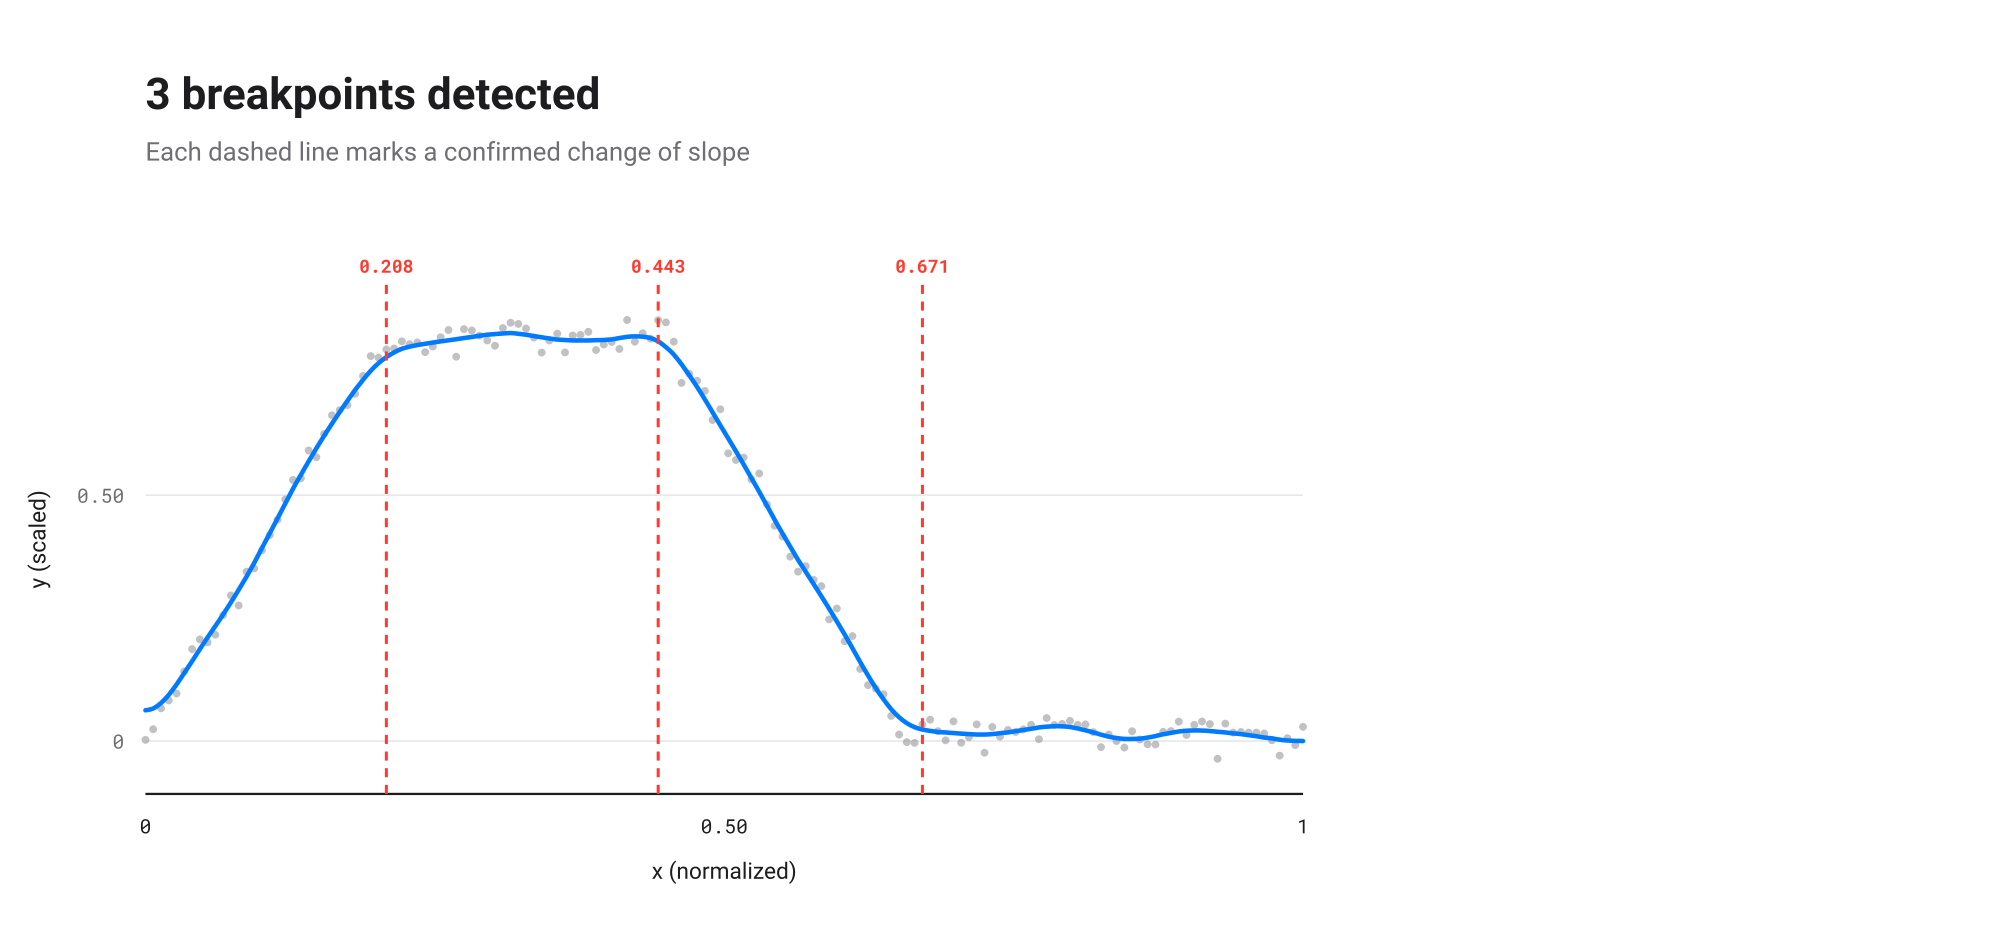
\includegraphics[width=0.8\textwidth]{figures/mountain_en.png}
\caption{A mountain curve with \code{elbow\_helper.robust\_knees}'s three
detected breakpoints (dashed red lines): up, flat, down, flat, recovered
without any curve/direction argument.}
\end{figure}

\part{One or several knees, with noise}
\label{part:noise}

Parts~\ref{part:one} and~\ref{part:several} describe the geometry of a bend
as if the data were exact. Real data never is, so nothing above is trusted
on its own. This part is the trust layer: a chain of independent checks a
single-knee candidate must survive to become a \code{ClearKnee}, and a set
of model-selection criteria that decide, for the multi-knee case, how many
breakpoints the noise actually supports.

\section{Is there even a trend? Spearman rank correlation}

\textbf{Intuition.} Before hunting for a knee, \code{elbow-helper} checks a
more basic question: does $y$ move consistently with $x$ at all? Not ``is
the relationship a straight line'' --- Pearson correlation asks that and
would be fooled by a genuine, curved knee shape --- but ``when $x$ goes up,
does $y$ tend to go up too, or down, however wiggly the path''. The trick is
to replace every value by its \emph{rank}, 1st smallest, 2nd smallest, and
so on, before correlating. Ranks discard exactly the information that would
make an ordinary correlation sensitive to the curve's exact shape or to
outliers, keeping only the ``does the order agree'' question.

\textbf{Worked example.} Five points with $x = (1,2,3,4,5)$ and $y =
(2,1,5,3,9)$. The $y$ ranks are $(2,1,3,4,5)$ (rank 1 is the smallest
value, so $y=1$ at position 2 gets rank 1, and so on). Even though the raw
values wiggle ($2, 1, 5, \dots$), the ranks track $x$'s ranks $(1,2,3,4,5)$
fairly closely, giving a high positive correlation despite the local dip.

\textbf{Formula.} With $r_i, s_i$ the ranks of $x_i, y_i$ (ties get the
average rank of the tied group):

\begin{equation}
\rho = \frac{\sum_i (r_i - \bar r)(s_i - \bar s)}{\sqrt{\sum_i (r_i - \bar r)^2}\ \sqrt{\sum_i (s_i - \bar s)^2}}
\end{equation}

\code{elbow\_helper.numerics.spearman} implements this directly (no
\code{scipy.stats.rankdata} dependency). A knee candidate is only screened
in if $|\rho|$ clears \code{config.min\_spearman\_abs} (default $0.60$) and
a magnitude-weighted ``how much of the movement fights the claimed
direction'' check also passes; see \code{INCOMPATIBLE\_GLOBAL\_SHAPE} in
the README's abstention-reason list \citep{spearman1904}.

\section{Not trusting one scale: the smoothing $\times$ sensitivity search}
\label{sec:multiscale}

\textbf{Intuition.} Look at a noisy curve at native resolution and every
little wiggle looks like a candidate knee. Smooth it heavily and a real
knee can get blurred away entirely. Neither extreme is trustworthy alone,
so \code{elbow-helper} runs the locator across a whole grid: several Gaussian
smoothing widths, from $1$, no smoothing, up to roughly a quarter of the
data, crossed with several sensitivities $S$. Every run that finds a knee
contributes one candidate to a pool; nothing is trusted yet, this stage
only \emph{proposes}.

\section{Only count it if it survives everywhere: persistence clustering}
\label{sec:persistence}

\textbf{Intuition.} A genuine knee should show up at nearly every smoothing
width and every sensitivity, wandering only slightly. A knee that is really
noise tends to jump around unpredictably as the smoothing changes, or shows
up at only one or two settings and vanishes elsewhere. \code{elbow-helper}
groups the candidate pool by location, within \code{cluster\_tolerance} of
each other, in normalized $x$ units, then asks of the largest group: does
it span several \emph{consecutive} smoothing scales, does it show up
across most sensitivities, is its spread (median absolute deviation)
tight? If two groups are both large and comparably supported, the pipeline
explicitly refuses to pick a winner (\code{MULTIPLE\_PLAUSIBLE\_KNEES}),
rather than guess (\code{src/elbow\_helper/\allowbreak clustering.py}).

\section{Confirming the slope: the Theil-Sen contrast}
\label{sec:theilsen}

\textbf{Intuition.} The ordinary way to estimate a slope, fit a line
through a bunch of points, is easily thrown off by a single bad point far
from the rest. The Theil-Sen estimator sidesteps this: compute the slope
between \emph{every pair} of points, then take the median of all those
slopes. A handful of bad pairs, involving an outlier, get outvoted by the
majority of good pairs.

\textbf{Worked example.} Three points $(0,0), (1,1), (2,100)$, the last one
a wild outlier. Pairwise slopes: $(1-0)/(1-0)=1$, $(100-0)/(2-0)=50$,
$(100-1)/(2-1)=99$. The median of $\{1, 50, 99\}$ is $50$, still pulled by
the outlier with only three points, but with more normal points and one
outlier, the median stops moving once outliers are a minority, unlike an
ordinary least-squares fit, which the outlier would dominate immediately.

\textbf{Formula.}

\begin{equation}
\hat\beta = \operatorname{median}_{i < j} \frac{y_j - y_i}{x_j - x_i}
\end{equation}

\code{elbow-helper} computes this on a small window just left and just
right of the candidate knee, then compares the two slopes:

\begin{equation}
\text{contrast} = \frac{|m_{\text{left}} - m_{\text{right}}|}{|m_{\text{left}}| + |m_{\text{right}}| + \epsilon}
\end{equation}

A contrast below \code{config.\allowbreak min\_slope\_contrast} (default $0.30$) fails
this check (\code{WEAK\_SLOPE\_CHANGE}) \citep{theil1950} \citep{sen1968}.

\section{Confirming the model: BIC and blocked cross-validation}
\label{sec:bic-cv}

\textbf{Intuition.} Every extra free parameter in a model can only help it
fit the \emph{training} data better, purely mechanically, whether or not it
captures anything real, a model with as many parameters as data points fits
perfectly and explains nothing. The Bayesian Information Criterion,
Schwarz's fix for this, charges each extra parameter a fixed toll, in units
of how much the log-likelihood must improve to be worth it, so that a model
is only preferred if it clears that bar.

\textbf{Where the log base comes from.} Section~\ref{sec:likelihood-intro}
derives, from the raw Gaussian likelihood $L(\theta,\sigma^2)$, that the
negative log-likelihood

\begin{equation}
\mathrm{NLL} = n \ln\!\left(\frac{RSS}{n}\right) + n(1 + \ln 2\pi)
\end{equation}

is natural-log by construction, inherited from the Gaussian density's own
$\exp$, not chosen freely, and that its extreme cases are best read
through $\mathrm{MSE}_{\text{worst}}$, a deliberately pessimistic finite
baseline, rather than through $\mathrm{MSE} \to \infty$ or the
easily-beaten sample mean. Every $\mathrm{BIC}$-family formula in this
note, including the one below, opens with this same $n\ln(RSS/n)$ term.

\textbf{Formula.} Schwarz's fix for the overfitting problem in this
section's Intuition paragraph adds a complexity penalty, $p \ln n$, on top
of this same $\mathrm{NLL}$, through a Laplace approximation to the
model's marginal likelihood carried out in the same natural log
throughout. Dropping the additive constant $n(1+\ln 2\pi)$, which cancels
when comparing two models on the same data:

\begin{equation}
\mathrm{BIC} = n \ln\!\left(\frac{RSS}{n}\right) + p \ln n
\end{equation}

Lower is better. \code{elbow\_helper.numerics.bic} implements exactly
this; the single-knee pipeline compares the $\mathrm{BIC}$ of the single
line ($p = 2 + 1$) against the broken line ($p = 3 + 1$) from Section~3,
requiring an improvement of at least \code{config.min\_bic\_improvement}
(default $10$) \citep{schwarz1978} \citep{hastie2009esl} \citep{bishop2006prml}.

\textbf{From $\Delta\mathrm{BIC}$ to a bounded score.} A raw
$\Delta\mathrm{BIC} = \mathrm{BIC}_{\text{single}} -
\mathrm{BIC}_{\text{broken}}$ has no natural ceiling: ``$10$'' and
``$282$'' both favour the broken line, but nothing about the number itself
says how confident that is; the scale shifts with sample size and noise
too. The diagnostic figure (\code{elbow\_helper.plotting}) instead reports
a probability, a score that must land in $[0, 1]$, with $0$ and $1$ as the
two extreme cases: total confidence in the single line or in the broken
one. That requirement is what fixes the log base, not a free
choice: \citet{kassraftery1995} (eq.~4) show
$\Delta\mathrm{BIC} \approx 2 \ln(\mathrm{BF})$, where $\mathrm{BF}$ is the
Bayes factor between the two models, and the $\ln$ on the right is the
\emph{same} natural log already used to build $\mathrm{BIC}$ above,
inherited from its $-2\ln(\hat L)$ definition. Undoing that $\ln$ therefore
needs the matching inverse, $\exp$ base $e$, not an arbitrary rescaling by
$\ln 10$ or $\ln 2$, which would only relabel an unbounded number, not
bound it:

\begin{equation}
\mathrm{BF} \approx \exp\!\left(\frac{\Delta\mathrm{BIC}}{2}\right)
\end{equation}

Under equal priors, posterior odds equal $\mathrm{BF}$, so the posterior
probability of the broken-line model is $\mathrm{BF} / (1 + \mathrm{BF})$,
which is exactly the logistic sigmoid of $\Delta\mathrm{BIC} / 2$:

\begin{equation}
P(\text{broken line} \mid \text{data}) = \frac{1}{1 + \exp(-\Delta\mathrm{BIC}/2)}
\end{equation}

bounded in $[0, 1]$ by construction, $0.5$ at $\Delta\mathrm{BIC} = 0$ (no
evidence either way), and saturating smoothly toward the $0$/$1$ extremes
as the evidence grows, in either direction, rather than growing without
limit the way the raw $\Delta\mathrm{BIC}$ does.

BIC only checks whether the extra parameter is worth its penalty \emph{on
the data used to fit it}. Blocked cross-validation asks a complementary,
more paranoid question: does the broken line still win when tested on data
it never saw while fitting? Ordinary shuffled cross-validation would leak
information here, since neighbouring points on a curve are similar, so
\code{elbow-helper} holds out \emph{contiguous} chunks of $x$ in turn, not
random points, mimicking how the curve would look with a genuine, unseen
chunk missing. This is the same validation-rigor concern Marcos L\'opez de
Prado's book on financial machine learning argues for at length, in the
context of ordered, sequential data \citeyearpar{lopezdeprado2018financial}.

\section{Bootstrap: does the knee survive a redo?}
\label{sec:bootstrap}

\textbf{Intuition.} If the data collection were repeated, would the same
knee show up again, or was this run's knee a fluke of this run's
particular noise? Since a real redo is not available, the bootstrap
simulates one: take the residuals left over after fitting the accepted
broken-line model, the part of $y$ the model did not explain, resample them
with replacement, add the resampled residuals back onto the fitted model to
build a synthetic ``redo'' curve, then rerun the \emph{entire} search on
it. Repeat many times, Efron's bootstrap. A knee that shows up only in the
original run, and rarely in the resampled redos, was probably a fluke.

\textbf{Formula.} For each of $B$ replicates, $y^\ast = \hat y + r^\ast$
where $r^\ast$ is a resample-with-replacement of the observed residuals.
\code{elbow-helper} requires the knee to be redetected in at least
\code{config.\allowbreak min\_bootstrap\_detection\_rate} (default $90\%$) of
replicates, with a tight, unimodal 90\% interval, the 5th-95th percentile
spread of the redetected locations \citep{efron1979} \citep{hastie2009esl}.

\section{The null test: could a straight line explain this by chance?}
\label{sec:null-test}

\textbf{Intuition.} The last, most skeptical check: simulate many curves
that have \emph{no} real knee at all, straight lines carrying noise at the
same estimated scale as the accepted model's residuals, run the exact same
search-and-confirm procedure on each, and count how often that procedure
still manages to report a knee as strong as the one actually observed. If
pure noise regularly produces something this strong, the observed knee is
not trustworthy evidence of a real bend, it is just what noisy straight
lines look like some of the time.

\textbf{Formula.} With $B = $ \code{config.null\_replicates} (default
$200$) Monte Carlo replicates and a lexicographic, search-adjusted test
statistic, so a null replicate only ``beats'' the observed knee if it
passes \emph{the same} confirmation gates, not just a raw score:

\begin{equation}
p = \frac{1 + \#\{\text{null replicates at least as strong as observed}\}}{B + 1}
\end{equation}

The $+1$ in numerator and denominator is the standard finite-sample
correction that keeps a Monte Carlo $p$-value from ever claiming exactly
zero. \code{elbow-helper} requires $p \le$ \code{config.\allowbreak max\_null\_p\_value}
(default $0.01$) (\code{src/elbow\_helper/\allowbreak null\_test.py}, whose own module
docstring states this exact formula).

Only a candidate that clears every check in the preceding sections becomes
a \code{ClearKnee}.

\section{Plain BIC for several knees: the naive criterion and why it overselects}
\label{sec:several-bic}

\textbf{Intuition.} Section~\ref{sec:bic-cv}'s BIC penalizes the number of
free \emph{regression} parameters, but choosing \emph{where} to place $k$
breakpoints among roughly $n$ possible positions is itself a form of
freedom, one that plain BIC never charges for. It is as if a
multiple-choice exam only docked points for wrong answers on the questions
attempted, ignoring how many questions there were to choose from in the
first place.

\textbf{Formula.} With $p = 2(k+1) + 1$, two regression parameters per
independent segment, plus the noise variance:

\begin{equation}
\mathrm{BIC}(k) = n \ln\!\left(\frac{RSS(k)}{n}\right) + p \ln n
\end{equation}

The consequence is not just theoretical: \code{RESULTS.md} measures a 27\%
false-positive rate for this exact criterion on data with no real
breakpoints and only 0.65 overall exact-$k$ accuracy, the worst of the
four criteria tested on the dynamic program's segmentations
\citep{yao1988} \citep{zhangsiegmund2007}.

The deeper reason plain BIC undercharges is that a breakpoint's location is
not a ``regular'' parameter in the technical sense BIC's derivation
assumes. The log-likelihood is not smooth, twice differentiable, in the
location, so the location estimator does not converge at the usual
$\sqrt n$ rate with a Gaussian limit; it converges faster, at rate $n$, with
a limiting distribution given by the argmax of a random walk. Charging
$\frac{1}{2}\ln n$ per parameter, the Laplace-approximation argument behind
BIC, assumes exactly the regularity that breaks down here.

\section{Modified BIC: Zhang and Siegmund's fix and a sign convention resolved by testing}
\label{sec:mbic}

\textbf{Intuition.} If plain BIC undercharges for the freedom to place
breakpoints, the fix is to charge more, specifically to charge \emph{more
for very short or very uneven segments}, since a tiny segment offers far
more placement freedom, many nearby positions all look almost as good, than
a segment that spans a large, well-defined chunk of the data.

\textbf{Formula.} Zhang and Siegmund's penalty, reported here through a
secondary source rather than the primary paper, is

\begin{equation}
\text{penalty}(k) = 3k \ln n + \sum_{j=1}^{k+1} \ln\!\left(\frac{\ell_j}{n}\right)
\end{equation}

where $\ell_j$ are the resulting segment lengths. The $3$, instead of plain
BIC's implicit $2$ from the two regression parameters alone, is already a
stronger complexity charge on its own; the second term is always $\le 0$
and, by the concavity of $\ln$, sits closest to zero when segments are
balanced and most negative when they are very uneven.

\textbf{A genuine ambiguity, resolved empirically rather than assumed.}
Folding this penalty into a lower-is-better criterion by direct addition,

\begin{equation}
\mathrm{mBIC}_{\text{additive}}(k) = n \ln\!\left(\frac{RSS(k)}{n}\right) + 3k \ln n + \sum_{j=1}^{k+1} \ln\!\left(\frac{\ell_j}{n}\right)
\end{equation}

makes the most-negative, uneven-segment case \emph{lower} the total, so this
combination \emph{rewards} uneven segments, the opposite of the
``penalizes short and uneven segments'' behaviour the term is meant to
have. Subtracting the same term instead,

\begin{equation}
\mathrm{mBIC}_{\text{subtractive}}(k) = n \ln\!\left(\frac{RSS(k)}{n}\right) + 3k \ln n - \sum_{j=1}^{k+1} \ln\!\left(\frac{\ell_j}{n}\right)
\end{equation}

does penalize uneven segments, matching the literature's stated intent.
Both forms are implemented and directly compared:
\code{modified\_bic\_subtractive} reaches 0.85 overall accuracy and a 0\%
false-positive rate at $\text{true } k = 0$; \code{modified\_bic\_additive}
still beats plain BIC (0.77 vs.\ 0.65) but leaves an 11\% false-positive
rate. \textbf{The subtractive form is the one shipped.}

\section{ICL: from mixture models to changepoints, including a bug this project found and fixed}
\label{sec:icl}

\textbf{Intuition.} Biernacki, Celeux and Govaert's Integrated Completed
Likelihood, developed for choosing the number of clusters in a mixture
model, adds one more consideration on top of BIC: not just ``does this
model fit well relative to its complexity'', but ``are the resulting
groups actually unambiguous''. Two overlapping, hard-to-tell-apart clusters
are penalized even if they fit the data about as well as two clean,
well-separated ones. Gilles Celeux, a co-author of the original ICL paper,
later co-wrote a book-length treatment of exactly this family of methods
\citep{bouveyron2021mbc}.

For changepoints, the analogue of ``which cluster does this point belong
to'' is ``where exactly is the cut'': the relevant uncertainty is over the
\emph{entire discrete segmentation}, not over individual point-to-component
labels. Rigaill, Lebarbier and Robin supply the machinery: an exact,
non-asymptotic posterior over every way to place $K-1$ breakpoints, via a
forward-backward dynamic program structurally identical to the
forward-backward algorithm of a Hidden Markov Model, run over segmentations
instead of hidden states \citeyearpar{rigaill2012}; Cleynen, Luong, Rigaill
and Nuel build directly on this \citeyearpar{cleynen2013}.

\textbf{Formula.} A forward pass computes, in log space, the total
likelihood mass over every valid $K$-segment partition of the first $t$
points, using the Gaussian segment log-likelihood

\begin{equation}
\ell\ell(i, j) = -\frac{RSS(i, j)}{2\sigma^2} - \frac{j - i}{2} \ln(2\pi\sigma^2)
\end{equation}
\begin{equation}
\log Z_1(t) = \ell\ell(0, t), \qquad \log Z_K(t) = \log \sum_{s} \exp\!\Big( \log Z_{K-1}(s) + \ell\ell(s, t) \Big)
\end{equation}

The entropy of the resulting discrete posterior over segmentations, $H(K) =
\log Z_K(n) - \mathbb{E}[\ell\ell(S)]$, is estimated by Monte Carlo
backward-sampling, drawing complete segmentations from the posterior and
averaging their log-probabilities, rather than derived in closed form.

\textbf{A bug the tests caught, not a design choice.} The first version
built here defined the score directly as $-\log Z_K(n) + H(K)$, pure
integrated likelihood plus entropy, no separate complexity penalty,
reasoning that the exact posterior already ``contains'' whatever complexity
notion is needed. Testing on sixty points of pure noise falsified that:
$\log Z_K(n)$ rose from 89.8 ($K=1$) to 94.7, 99.0, and 102.8 nats as $K$
grew to 4, purely from summing over combinatorially more candidate
segmentations, while entropy only rose from 0 to 3.7, 5.9, and 7.9 nats
over the same steps, not fast enough to cancel the growth. The resulting
score kept improving as $K$ grew even on flat noise, exactly the
overselection failure this whole exercise exists to avoid.

The fix follows from re-reading the mixture-model form above: ICL is
\emph{BIC plus} an entropy correction, not a replacement for BIC's own
complexity penalty:

\begin{equation}
\mathrm{ICL}(k) = \mathrm{BIC}(k) + 2\,H(K), \qquad K = k+1
\end{equation}

Retested on the same flat-noise data, this version correctly selects $k =
0$; \code{RESULTS.md} shows it performing in the same tier as the
subtractive mBIC (0.82 vs.\ 0.85 overall accuracy) once corrected
\citep{biernacki2000}.

\textbf{One log base, top to bottom.} The Gaussian segment log-likelihood
$\ell\ell(i,j)$ above, plain $\mathrm{BIC}(k)$ (Section~\ref{sec:several-bic}),
$\mathrm{mBIC}_{\text{subtractive}}(k)$, and $\mathrm{ICL}(k) =
\mathrm{BIC}(k) + 2H(K)$ are all written in \emph{natural} log throughout
this project's implementation, \code{numerics.py}'s single-knee
$\mathrm{BIC}$, \code{multi\_criteria.py}'s $\mathrm{mBIC}$, and
\code{research/multiknee/criteria.py}'s $\ell\ell$ / $\log Z_K$ / ICL all
call \code{np.log}, never \code{np.log10} or \code{np.log2}. That is not
an implementation detail to normalize away: it is exactly what makes
Section~\ref{sec:bic-cv}'s $\Delta\mathrm{BIC} \approx 2\ln(\mathrm{BF})$
argument and the $\exp$-then-sigmoid conversion into a $[0,1]$-bounded
posterior probability built on it apply unchanged to a difference between
any two of these four quantities, not only to plain single-knee
$\mathrm{BIC}$. $\Delta\mathrm{mBIC}$ or $\Delta\mathrm{ICL}$ between two
candidate segmentations is, by the same substitution, $2\ln$ of an
approximate Bayes factor between them, so the identical base-$e$
$\exp(\cdot/2)$ and logistic-sigmoid steps turn it into a bounded
confidence score, with $0$ and $1$ the same two extreme cases as before.
\code{elbow-helper} does not ship this conversion for the multi-knee
criteria (the shipped pipeline gates $k$ via the FWER test of the next
section instead), but the derivation carries over exactly, because the log
base was never a free choice to begin with.

\section{A sequential test controlling the family-wise error rate}
\label{sec:fwer}

\textbf{Intuition.} Independent of any BIC-family score, a more direct
question can be asked at each step: walking the sequence of segmentations
$k = 1, 2, \dots$, is the error reduction from adding breakpoint $k$ bigger
than pure chance would produce? This is answered the way a permutation
test answers any such question: resample what ``chance'' looks like many
times and see how often chance alone beats what was actually observed.

\textbf{Formula.} At each step, residuals $r = y - \hat y_{k-1}$ under the
accepted $(k-1)$-breakpoint model are resampled with replacement, Efron's
bootstrap again, to build $B$ synthetic curves $y^\ast = \hat y_{k-1} +
r^\ast$. On each, the largest possible error reduction from one more split
anywhere is computed, giving a null distribution:

\begin{equation}
p = \frac{1 + \#\{\text{replicates with null reduction} \ge \text{observed reduction}\}}{B + 1}
\end{equation}

Breakpoint $k$ is accepted only if $p \le \alpha / k_{\max}$, a Bonferroni
correction across up to $k_{\max}$ sequential tests. The procedure stops at
the first breakpoint that fails, so it can never ``skip'' a rejected
breakpoint and accept a later one. Bonferroni is conservative for
independent tests; these sequential tests are not independent, each
conditions on the model accepted at the previous step, which keeps the
true family-wise error rate (FWER), the probability of accepting at
least one spurious breakpoint anywhere in the sequence, at most as large
as the nominal $\alpha$, not larger.

\code{RESULTS.md} shows this reaching a 0\% false-positive rate at
$\text{true } k = 0$ and 0.82 overall accuracy, in the same tier as the
subtractive mBIC and the corrected ICL. Two more rigorous alternatives were
considered and not implemented: Davies' asymptotic test
\citeyearpar{davies1977} and the multiscale guarantee of SMUCE,
``Simultaneous MUlti-scale Change-point Estimator'' \citep{frick2014}, in
favour of a permutation test whose correctness is checkable directly by
simulation.

\section{Where this leaves the shipped API}

\code{elbow\_helper.robust\_knees} ships exactly the combination validated
above: dynamic-program search (Section~\ref{sec:dp}), the subtractive-sign
modified BIC as the primary criterion (Section~18), and the FWER
sequential gate (Section~20) layered on top by default, taking
$\min(\text{mBIC's } k,\ \text{FWER's } k)$, matching \code{elbow-helper}'s
stated design priority of minimizing false-positive knees even at the cost
of more abstentions. Plain BIC, the additive mBIC, ICL, and greedy search
are kept in \code{research/multiknee/} as tested-and-rejected, or
tested-and-costly, alternatives that justify that choice, not shipped as
public configuration options, so the public API surface reflects what was
actually shown to work.

\section{A worked example: a sigmoid staircase}

Every section above is either a formula or a claim checked by a test. Here
is one curve, run through the actual shipped code, to see the whole chain
land somewhere concrete.

A logistic sigmoid, $1/(1+e^{-\text{steepness}(x-\text{center})})$, rises
smoothly from 0 to 1 around its center and has no literal breakpoint
anywhere: it is infinitely differentiable, with no kink for a
piecewise-linear search to latch onto in principle. Summing three sigmoids
at different centers, each scaled to add one ``step'', builds a smooth
staircase: three rises separated by flat plateaus, the kind of shape that
shows up whenever several independent thresholds get crossed in sequence,
three separate user cohorts each ramping up adoption in a different week,
three separate sensors each saturating at a different load.

A piecewise-\emph{linear} model, run against a smooth curve like this,
cannot represent a rise with a single straight segment without either
cutting a flat plateau short or cutting the rise short. The compromise
\code{robust\_knees} settles on is visible directly in the figure below:
each of the three rises gets bracketed by \emph{two} breakpoints, one where
the flat plateau ends and the rise begins, one where the rise ends and the
next plateau begins. Three rises, six breakpoints, no exceptions across
five different noise draws tested
(\code{tests/test\_multiknee.py::\allowbreak test\_sigmoid\_staircase\_brackets[...]breakpoint\_pair}).

\begin{figure}[h]
\centering
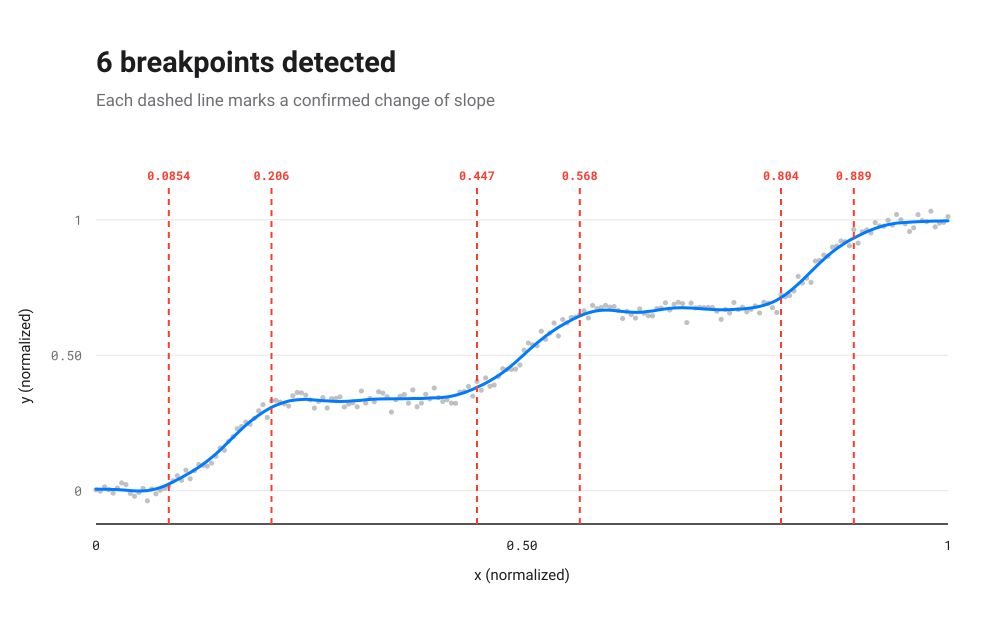
\includegraphics[width=0.8\textwidth]{figures/sigmoid_staircase_en.png}
\caption{A smooth staircase built from three logistic sigmoids, with
\code{elbow\_helper.robust\_knees}'s six detected breakpoints (dashed red
lines) each bracketing one rise's start and end.}
\end{figure}

One practical trap this example surfaced, worth stating plainly: the FWER
gate's Bonferroni correction divides $\alpha$ by $k_{\max}$, so the smallest
$p$-value the permutation test can produce, $1/(n_{\text{permutations}}+1)$,
must stay below $\alpha/k_{\max}$, or the gate can never pass no matter how
real the effect is. With the default $k_{\max}=4$ and
$\text{fwer\_permutations}=200$, $1/201 \approx 0.005 < 0.05/4 = 0.0125$,
comfortably clear. Push $k_{\max}$ up, as this six-breakpoint example
needs, without also raising \code{fwer\_permutations}, and the gate
silently locks itself out: this is exactly what happened on the first
attempt at this example ($k_{\max}=8$, the default 100 permutations, every
single breakpoint rejected with $k=0$), caught by looking at the
diagnostics rather than assuming the algorithm had failed for some more
mysterious reason.

\section{A worked example: the same subtle knee, at two noise levels}

Every check in Sections~\ref{sec:multiscale}--\ref{sec:null-test} exists to
answer one question honestly: is this knee real, or is it what noise looks
like sometimes? The cleanest way to see the answer is to hold the true
shape fixed and only change the noise.

\code{tests/test\_multiknee.py::subtle\_knee\_curve} is deliberately
unspectacular: a small, genuine slope change at $x = 0.5$, nowhere near as
dramatic as the sigmoid staircase or the mountain. At low noise,
\code{robust\_knees} detects it reliably, on every seed tested. At high
noise, with the identical true shape underneath, it mostly abstains,
reporting zero breakpoints rather than a guess.

\begin{figure}[h]
\centering
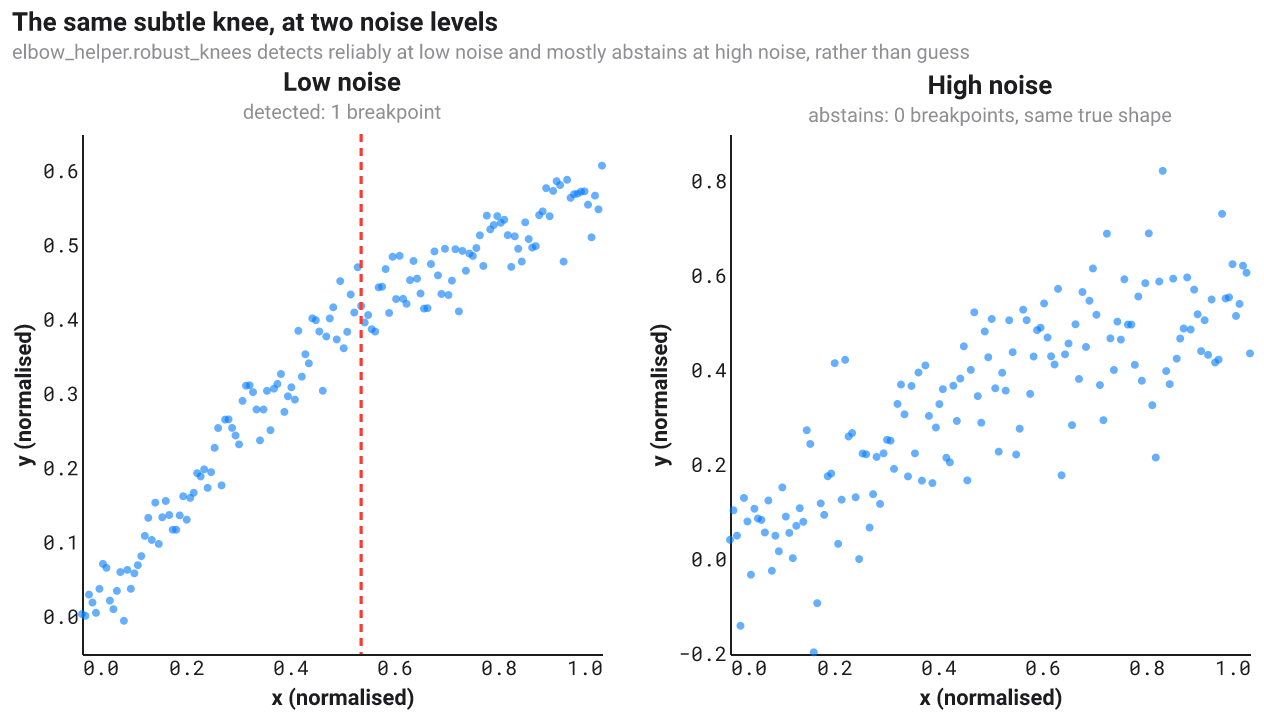
\includegraphics[width=0.8\textwidth]{figures/subtle_knee_en.png}
\caption{The same subtle knee at two noise levels: low noise (left) is
detected with one breakpoint, high noise (right) abstains with zero, the
same true shape underneath both panels.}
\end{figure}

This is the design priority from Section~21 made visible on one curve:
\code{elbow-helper} is built to be wrong in the honest direction. A missed
real knee at high noise is a cost this library accepts deliberately; a
reported knee that is really noise is the failure mode every check in
Part~\ref{part:noise} exists to rule out.

\section{A worked example: the PCA scree plot}

The other case \code{robust\_elbow}'s docstring names directly: a scree
plot, the eigenvalues of a covariance matrix in decreasing order, used to
decide how many principal components carry real signal versus noise.

\code{tests/test\_real\_world\_examples.py::pca\_scree\_curve} builds data
with six genuine signal dimensions (large variance) buried in nineteen
noise dimensions, rotated so the signal is not aligned with any one
measured axis, the setting PCA itself is built to unmix. The noise
dimensions are not equal-variance: their variance decays geometrically, the
shape a real Marchenko-Pastur noise spectrum actually takes, not the flat
block a first pass at this example produced before that mismatch was
caught. The resulting eigenvalue curve drops by an order of magnitude
exactly at the signal/noise boundary, then keeps decaying, slowly and
smoothly, rather than levelling into a plateau.

\begin{figure}[h]
\centering
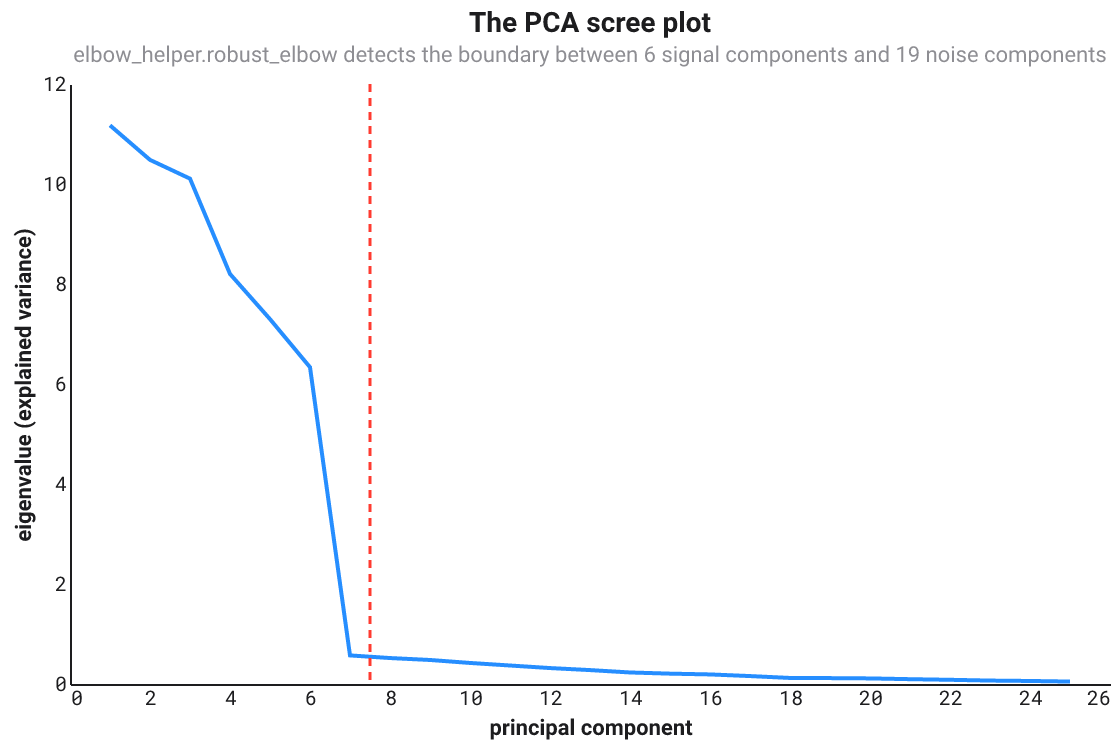
\includegraphics[width=0.8\textwidth]{figures/pca_en.png}
\caption{The PCA scree plot, with \code{elbow\_helper.robust\_elbow}'s
detected elbow (dashed red line) at the boundary between 6 signal
components and 19 noise components.}
\end{figure}

This example shares Section~4's practical trap exactly: a scree plot is
short and left-heavy in precisely the same way an inertia curve is, so it
needs the same relaxed \code{RobustKneeConfig} profile. It also surfaces
the convention worth knowing about before reading \code{knee\_x} off any
short applied curve: the locator's ``last point before the bend'' rule
consistently lands one to two components \emph{past} the last true signal
component, not exactly on it. Across every seed tested, the detected elbow
falls at 6 or 7 components for a true signal dimension of 6, never below
it, a systematic, predictable offset rather than noise.

\section*{Further reading}

For a deeper or more rigorous treatment of the ideas above than this note
attempts, not as sources of any specific claim already cited, but as
places to go further:

\begin{itemize}[leftmargin=*]
\item Hastie, Tibshirani and Friedman on the bias-variance trade-offs
  behind BIC, cross-validation and the bootstrap \citeyearpar{hastie2009esl}
\item Bishop on the Bayesian model-selection framing that motivates BIC and
  ICL \citeyearpar{bishop2006prml}
\item Bouveyron, Celeux, Murphy and Raftery on mixture models and
  model-based clustering at book length \citeyearpar{bouveyron2021mbc}
\item Cormen, Leiserson, Rivest and Stein on dynamic programming in general
  \citeyearpar{cormen2022algorithms}
\item Dasgupta, Papadimitriou and Vazirani on dynamic programming again,
  leaner and intuition-first: this project's own favourite treatment of the
  recursion behind Section~\ref{sec:dp} \citeyearpar{dasgupta2006algorithms}
\item L\'opez de Prado on validation rigor for ordered, sequential data
  \citeyearpar{lopezdeprado2018financial}
\end{itemize}

\bibliography{references}

\end{document}
